\documentclass[11pt,a4paper]{article}
 
%-----------MATEMATYKA----------------------------------------
\usepackage{array}
\usepackage{amsmath}
\usepackage{amssymb}
%-------------------------------------------------------------

%\usepackage{multiline}
\usepackage{changepage}
\usepackage{geometry}
\newgeometry{tmargin=2.5cm, bmargin=3.5cm, lmargin=3.5cm, rmargin=3.5cm}

\usepackage{indentfirst}
\usepackage{graphicx} 	
\usepackage{float}
\usepackage[utf8]{inputenc} 
\usepackage[english,polish]{babel}
\usepackage{polski}

%------------ HYPERREF----------------------------------------
\usepackage{hyperref}
% tu można dodać \usepackage{caption} dla figure gez caption
\usepackage[all]{hypcap} % odnośniki do góry figure

\usepackage{xcolor}  
\hypersetup{         %stylowe hyperrefy zamiast czerwonych ramek
    colorlinks,
    linkcolor={red!50!black},
    citecolor={blue!50!black},
    urlcolor={blue!80!black}
}
%-------------------------------------------------------------


\title{Teoria optymalizacji - sprawozdanie z projektu}
\author{Piotr Dulewicz 209253 \\ Konrad Pleban numerindeksu \\ Termin zajęć: poniedziałek parzysty 11:15 \(-\) 13:00}
\date{}

\begin{document}
\maketitle
\section{Sformułowanie zadania optymalizacji}
Zadanie projektowe polegało na dwukryterialnej optymalizacji funkcji nieliniowych z użyciem algorytmu genetycznego NSGA. W programie zaimplementowana została jego nowsza wersja, o lepszej złożoności obliczeniowej, nazwana NSGA-II \cite{deb}. Wymiar zadania ustalony został jako \(n \leqslant 10\). Jedyne ograniczenia nałożone były na wektor zmiennych decyzyjnych, i miały postać
\[
X =  \lbrace x : L_i \leqslant x_i \leqslant U_i \rbrace, ~~~ i = 1,2,... ,n,  
\]
gdzie symbole \(L_i\) i \(U_i\) oznaczają odpowiednio dolne i górne ograniczenie dla \(i-\)tej zmiennej decyzyjnej. Funkcja celu, której minimum poszukiwane było przez algorytm, miała postać
\begin{equation}
F(x) = \begin{bmatrix}
  f_1(x) \\
  f_2(x) 
 \end{bmatrix}.
\label{eq:funkcja_celu}
\end{equation}

\section{Omówienie algorytmu optymalizacji}
Aby skutecznie poszukiwać minimum funkcji opisanej wyrażeniem (\ref{eq:funkcja_celu}), należy najpierw określić jak w ogóle rozumieć minimum, gdy funkcja zwraca więcej niż jedną wartość. Rozpatrzmy przypadek dwukryterialny. Za optymalne przyjmuje się każde niezdominowane rozwiązanie. Wszystkie optymalne rozwiązania są tak samo dobre, poszukiwane jest więc nie jedno minimum, a cały ich zbiór, zwany zbiorem Pareto (lub frontem Pareto). Rozwiązanie zdominowane to takie, dla którego istnieje rozwiązanie lepsze względem jednej z funkcji \(f(x)\), i nie gorsze względem drugiej. Wszystkie pozostałe rozwiązania są niezdominowane. 

Pierwszym krokiem algorytmu jest wygenerowanie losowej populacji, równomiernie rozłożonej na całym zbiorze rozwiązań dopuszczalnych \(X\). Następnie populacja dzielona jest na kolejne fronty Pareto. Do pierwszego frontu należeć będą wszystkie rozwiązania niezdominowane. Drugi front stanowią rozwiązania, które zdominowane są jedynie przez elementy pierwszego frontu. Kolejne fronty tworzone są w analogiczny sposób, aż do pełnej segregacji całej populacji. Im mniejszy jest numer frontu, do którego przydzielone zostało rozwiązanie, tym większy jest jego wskaźnik przystosowania, na podstawie którego wybierani są rodzice, którzy utworzą potomstwo w kolejnym kroku. Selekcja odbywa się za pomocą prostego turnieju binarnego. Rozwiązania, które przejdą przez ten etap są ze sobą losowo parowane, i następuje krzyżowanie. Polega ono na obliczeniu średniej ważonej dwóch rozwiązań, przy czym jeden z rodziców ma większą wagę. Każda para tworzy dwa nowe rozwiązania, w każdym z nich, inny rodzic jest tym dominującym. W ten sposób uzyskiwana jest pewna różnorodność. Następnie, z zadanym prawdopodobieństwem następuje mutacja rozwiązania. Jego składowe zmieniają się wtedy o niewielki procent. 

Po wygenerowaniu potomstwa, populacja dwukrotnie zwiększa swoją objętość. Następuje ponowna segregacja rozwiązań na kolejne fronty Pareto. Pośród poszczególnych frontów, rozwiązania oceniane są jeszcze ze względu na zagęszczenie. Wyżej oceniane są te, których odległość od sąsiednich rozwiązań jest duża. W ten sposób zapobiega się ich zbytniej koncentracji, natomiast preferuje się szerokie fronty, dobrze obrazujące granicę optymalnych rozwiązań. Na koniec odrzucana jest gorzej przystosowana połowa populacji, i algorytm wraca do punktu sprzed wydania potomstwa. Cykl ten powtarza się \(L\) razy, gdzie \(L\) jest ustaloną przez użytkownika liczbą generacji.

\section{Informacje o programie}
Program został napisany w języku C++, z użyciem biblioteki graficznej Qt, w środowisku Qt Creator. Do wizualizacji zbioru Pareto w przestrzeni funkcyjnej użyta została klasa QCustomPlot. Jej autorem jest Emanuel Eichhammer. Narzędzie to udostępnione jest na licencji GNU GPL pod adresem \url{http://www.qcustomplot.com/index.php/}. Do interpretacji wyrażeń matematycznych skorzystano z biblioteki \textit{C++ Mathematical Expression Toolkit}. Jej autorem jest Arash Partow. Biblioteka jest dostępna na licencji MIT pod adresem 
\url{http://partow.net/programming/exprtk/index.html}. 

\begin{figure}[H]
\centering
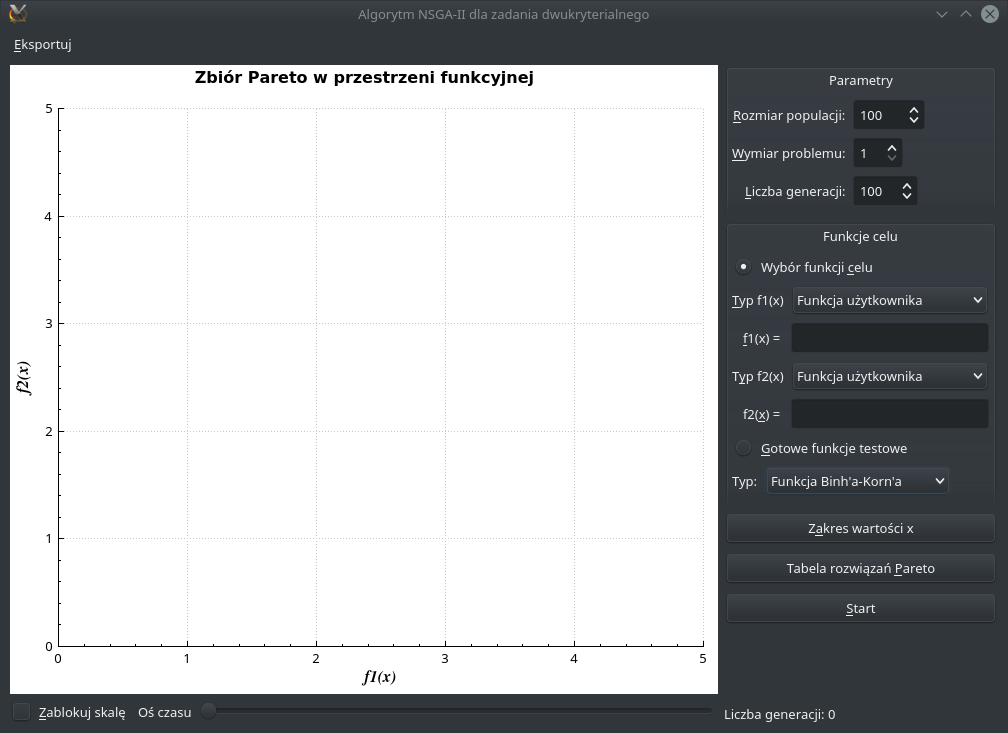
\includegraphics[width=14cm]{program}
\caption{Główne okno programu}
\label{fig:program}
\end{figure}

Na rysunku \ref{fig:program} widoczne są główne funkcjonalności programu. Po prawej stronie znajduje się panel sterowania. W sekcji \textit{Parametry} użytkownik może ustalić rozmiar populacji, wymiar problemu, oraz liczbę generacji. Nieco niżej umieszczona została sekcja o nazwie \textit{Funkcje celu}. Pozwala ona użytkownikowi na wprowadzenie własnych funkcji \(f_1(x)\) i \(f_2(x)\), za pomocą wyrażeń matematycznych akceptowanych przez parser. Ze względu na użycie biblioteki \textit{C++ Mathematical Expression Toolkit}, wyrażenia te mogą być bardzo różnorodne. Rozpoznawane są funkcje takie jak \textit{exp, abs, sqrt, floor}, dzielenie modulo, logarytmy o różnych podstawach, potęgi, czy też praktycznie wszystkie popularne funkcje trygonometryczne. Oprócz wpisania własnego wyrażenia, istnieje możliwość wyboru przygotowanych wcześniej funkcji  Rosenbrock'a,  Ackley'a,  Rastrigina i Goldsteina-Price'a. Dodatkowo, po zaznaczeniu opcji \textit{Gotowe funkcje testowe}, użytkownik może wybrać jedną z przygotowanych dwukryterialnych funkcji \(F(x)\), są to funkcja Binh'a-Korn'a, funkcja Fonseca-Fleminga oraz funkcja Kursawe.

Zlokalizowane niżej przyciski pozwalają zmienić zakres wartości zmiennych decyzyjnych, przejrzeć tabelę rozwiązań Pareto, oraz uruchomić algorytm. Pod wykresem umieszczona została oś czasu, pozwalająca na prześledzenie klatka po klatce kształtowania się optymalnego rozwiązania w kolejnych generacjach. Obok osi wyświetlana jest aktualna liczba generacji. 

\section{Przykłady testowe}
% dopisać tu tekst
\begin{figure}[H]
\centering
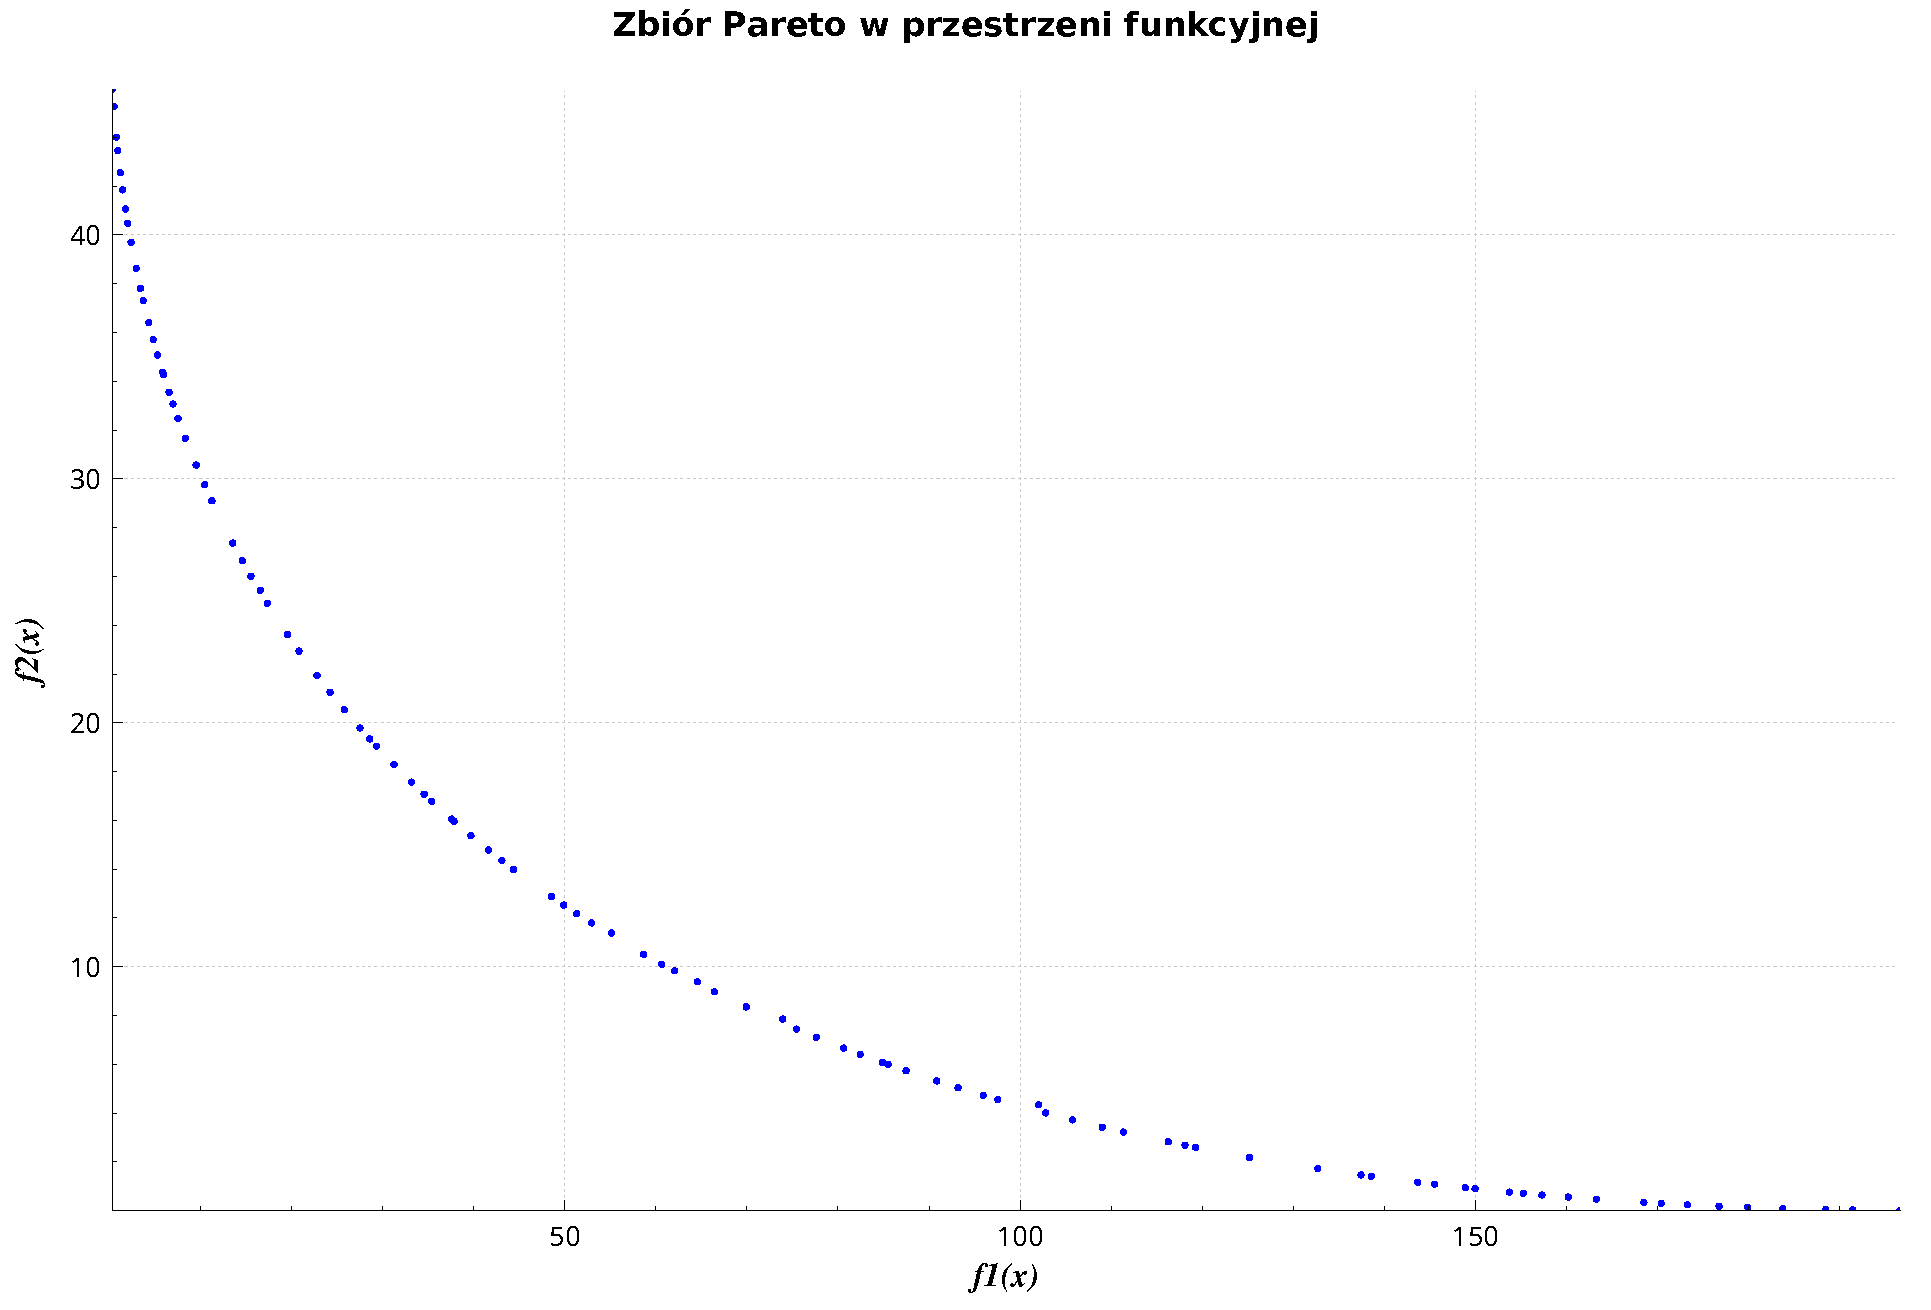
\includegraphics[width=14cm]{binh_korn_100_100}
\caption{TBD}
\label{fig:binh_korn_100_100}
\end{figure}

\begin{figure}[H]
\centering
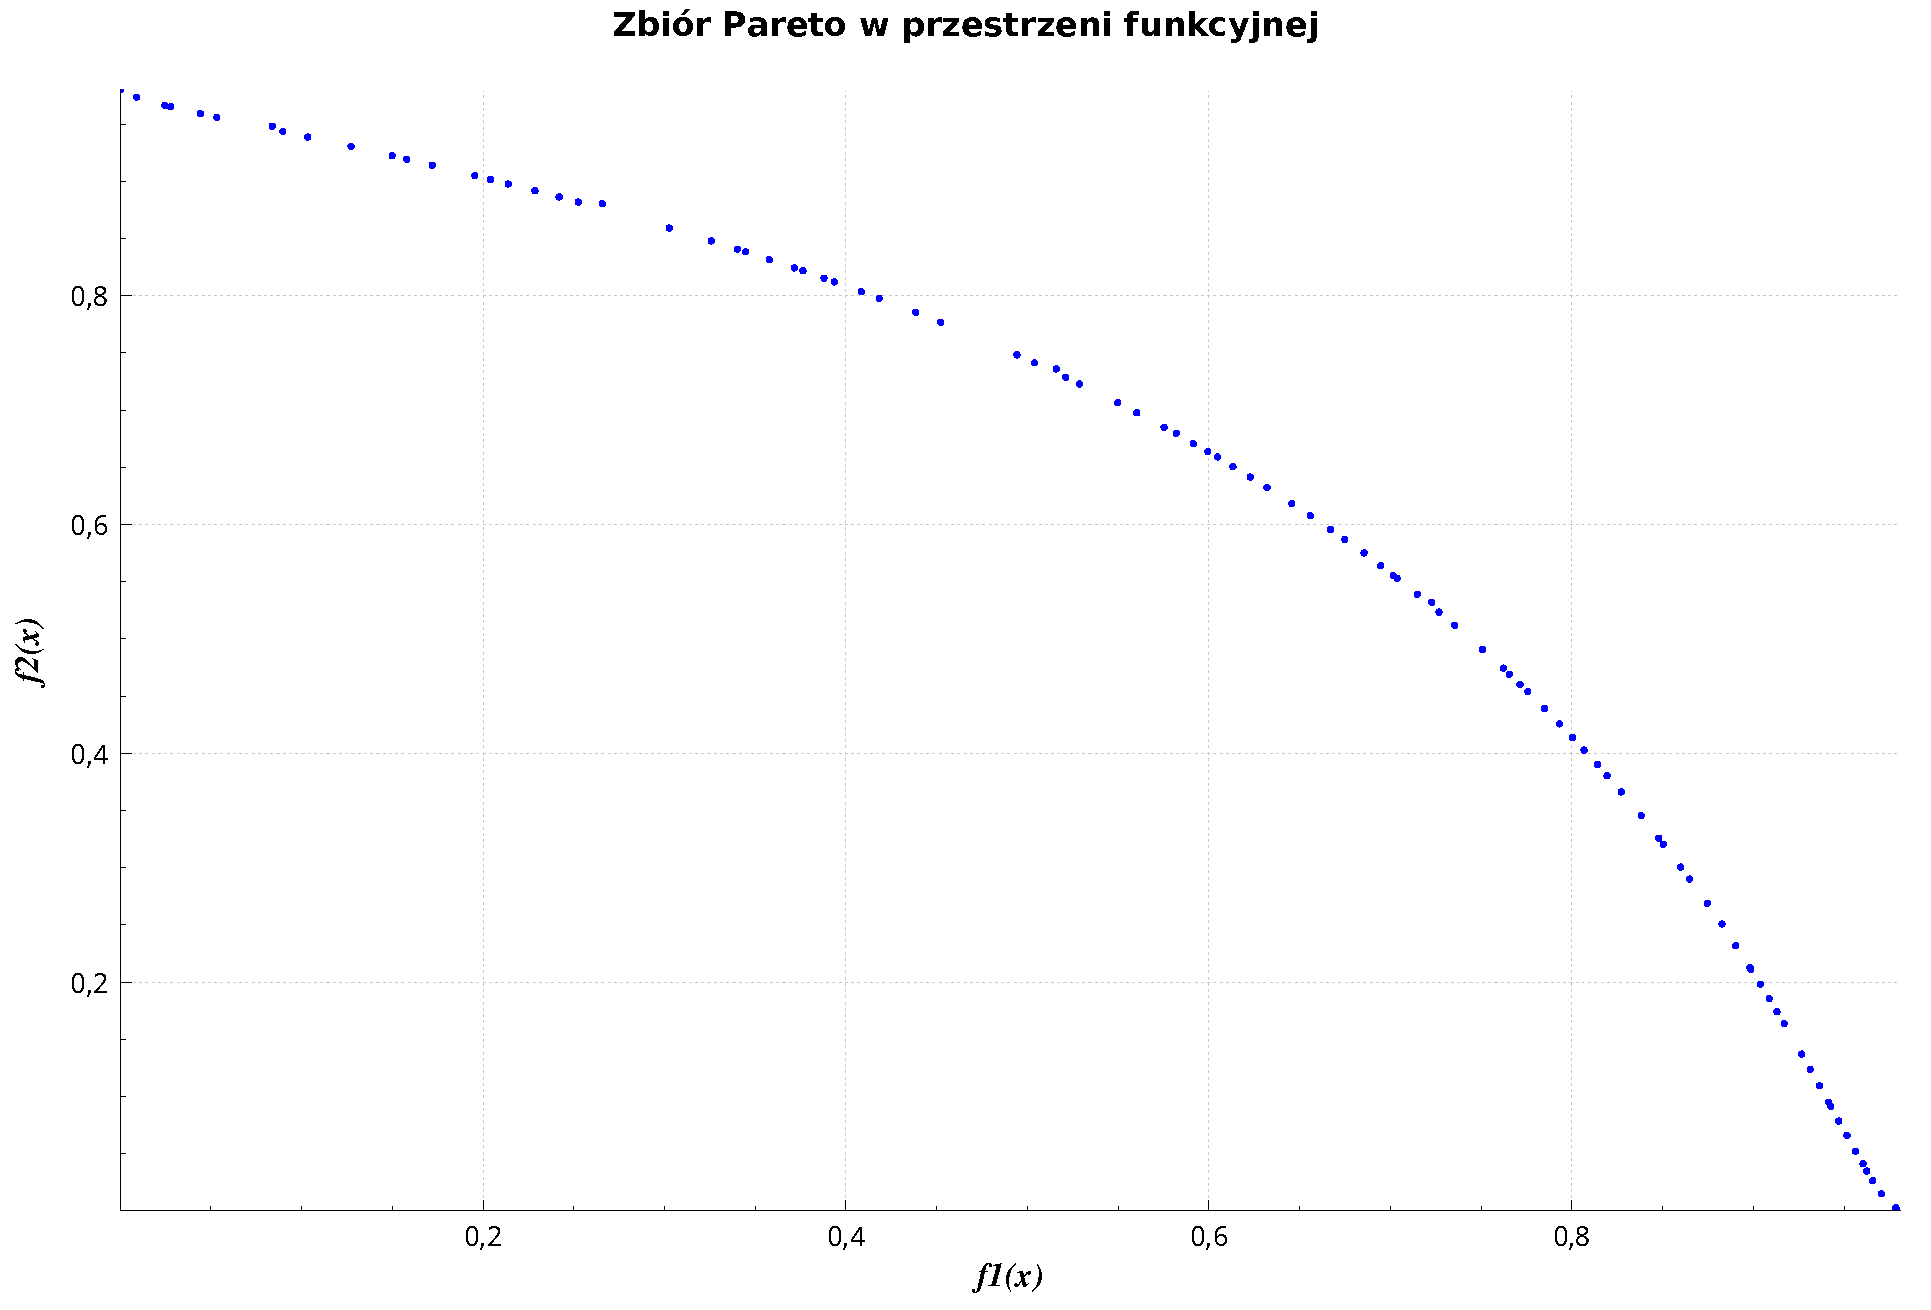
\includegraphics[width=14cm]{fonsec_fleming_100_100}
\caption{TBD}
\label{fig:fonsec_fleming_100_100}
\end{figure}

\begin{figure}[H]
\centering
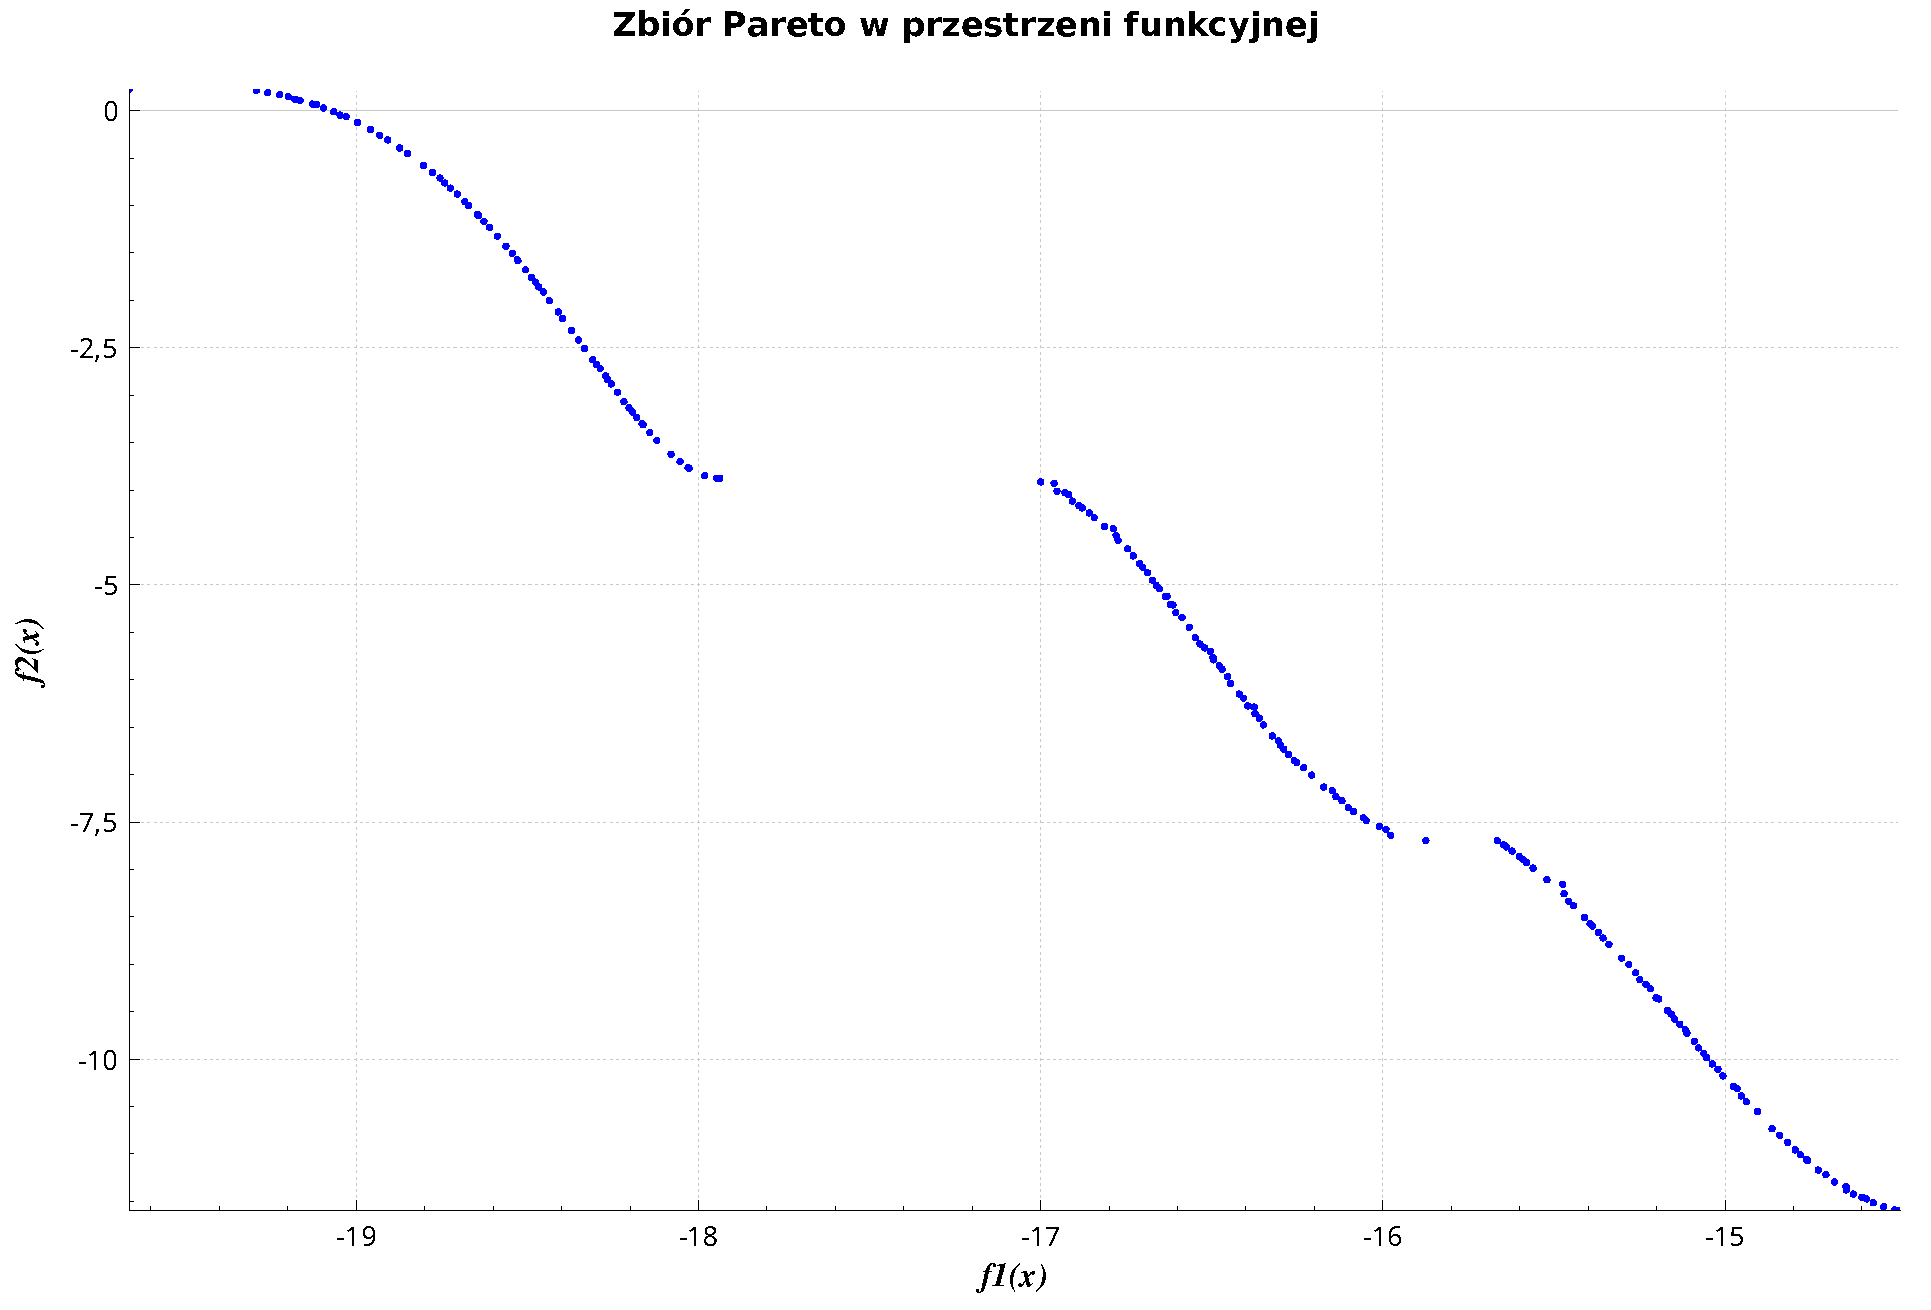
\includegraphics[width=14cm]{kursawe_200_100}
\caption{TBD}
\label{fig:kursawe_200_100}
\end{figure}

\begin{figure}[H]
\centering
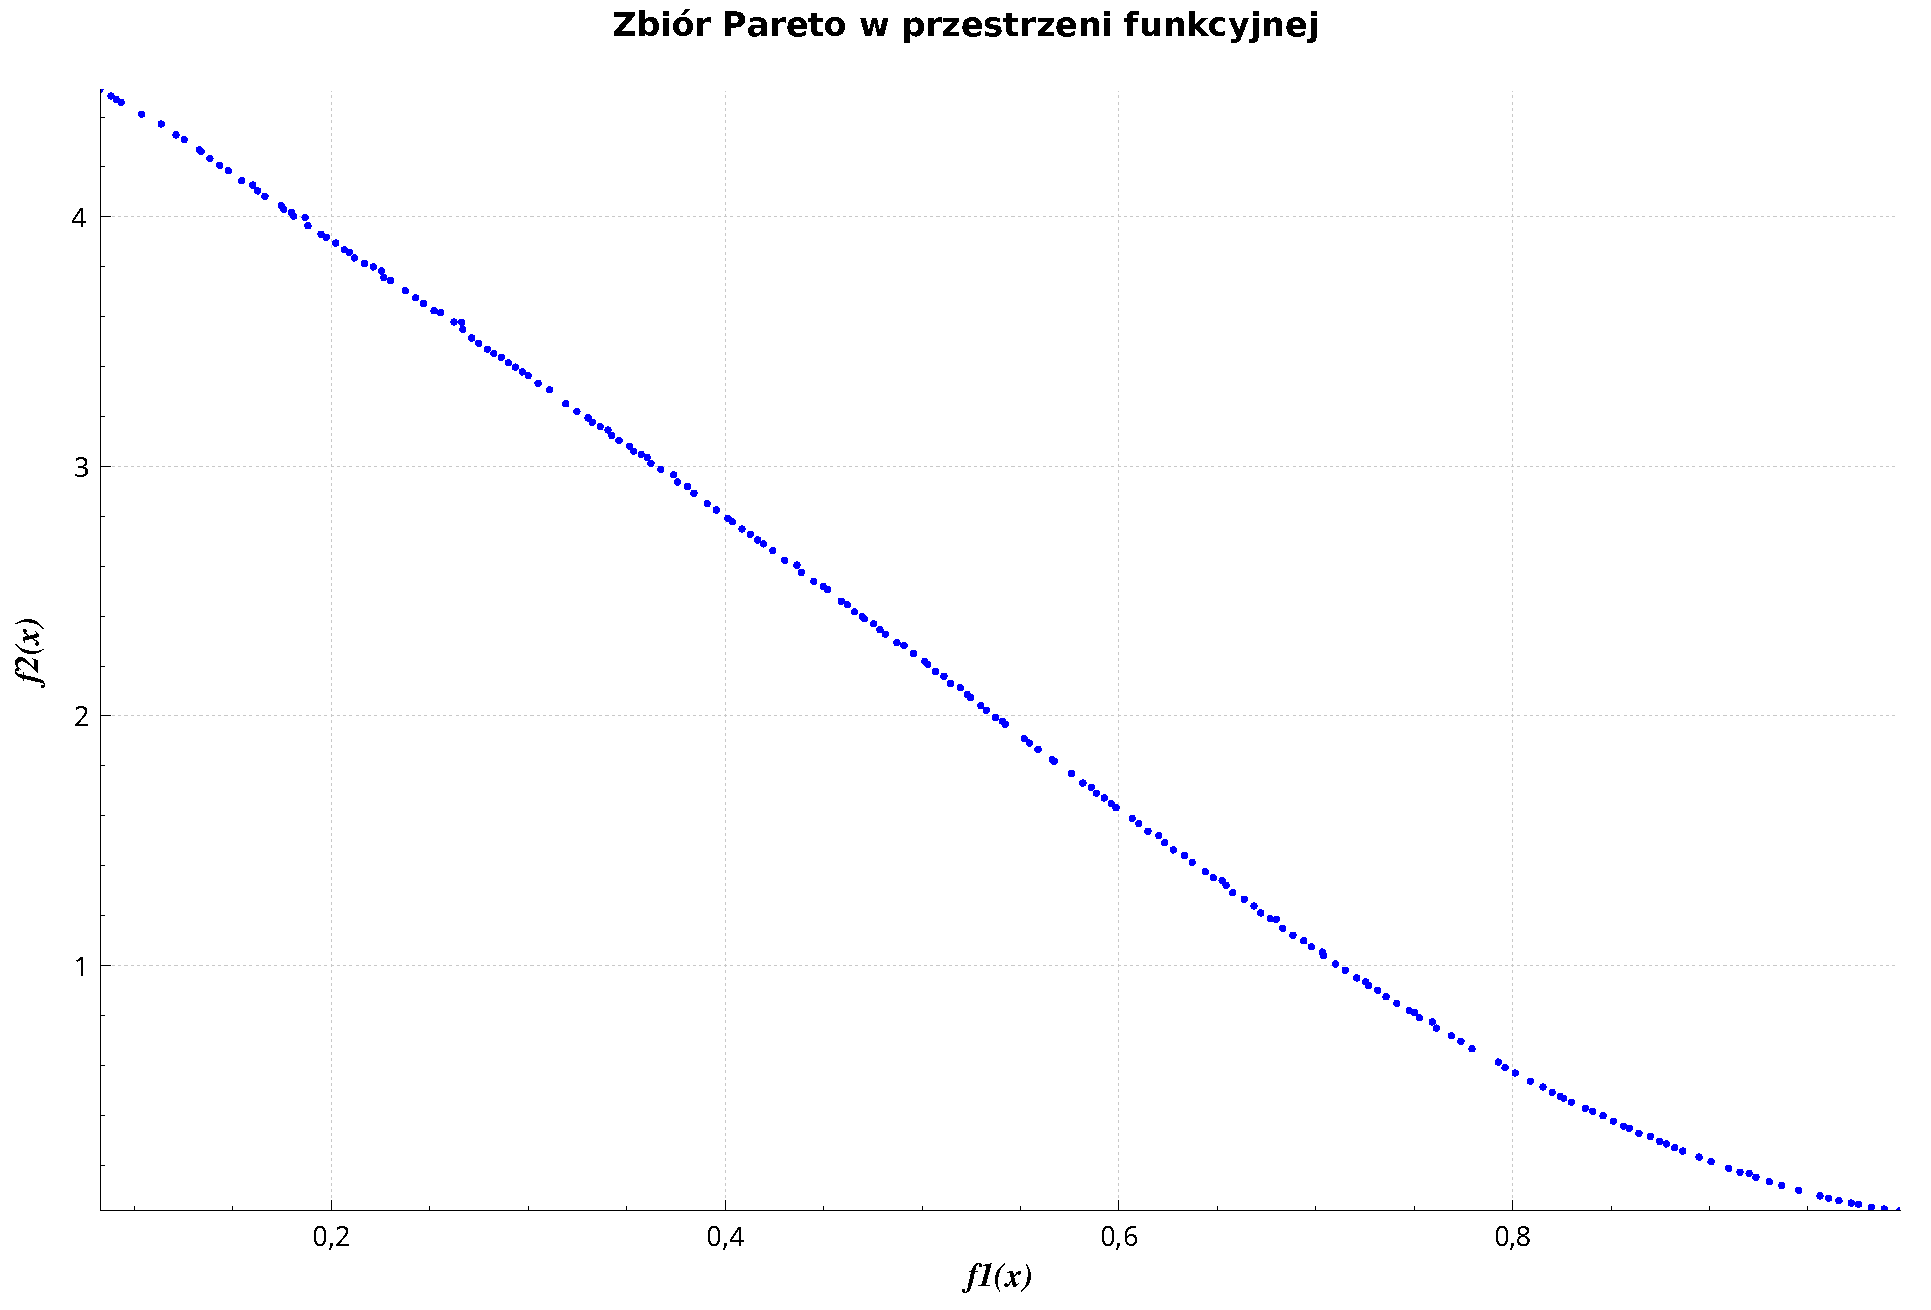
\includegraphics[width=14cm]{rosenbrock_ackley_200_100}
\caption{TBD}
\label{fig:rosenbrock_ackley_200_100}
\end{figure}

\begin{figure}[H]
\centering
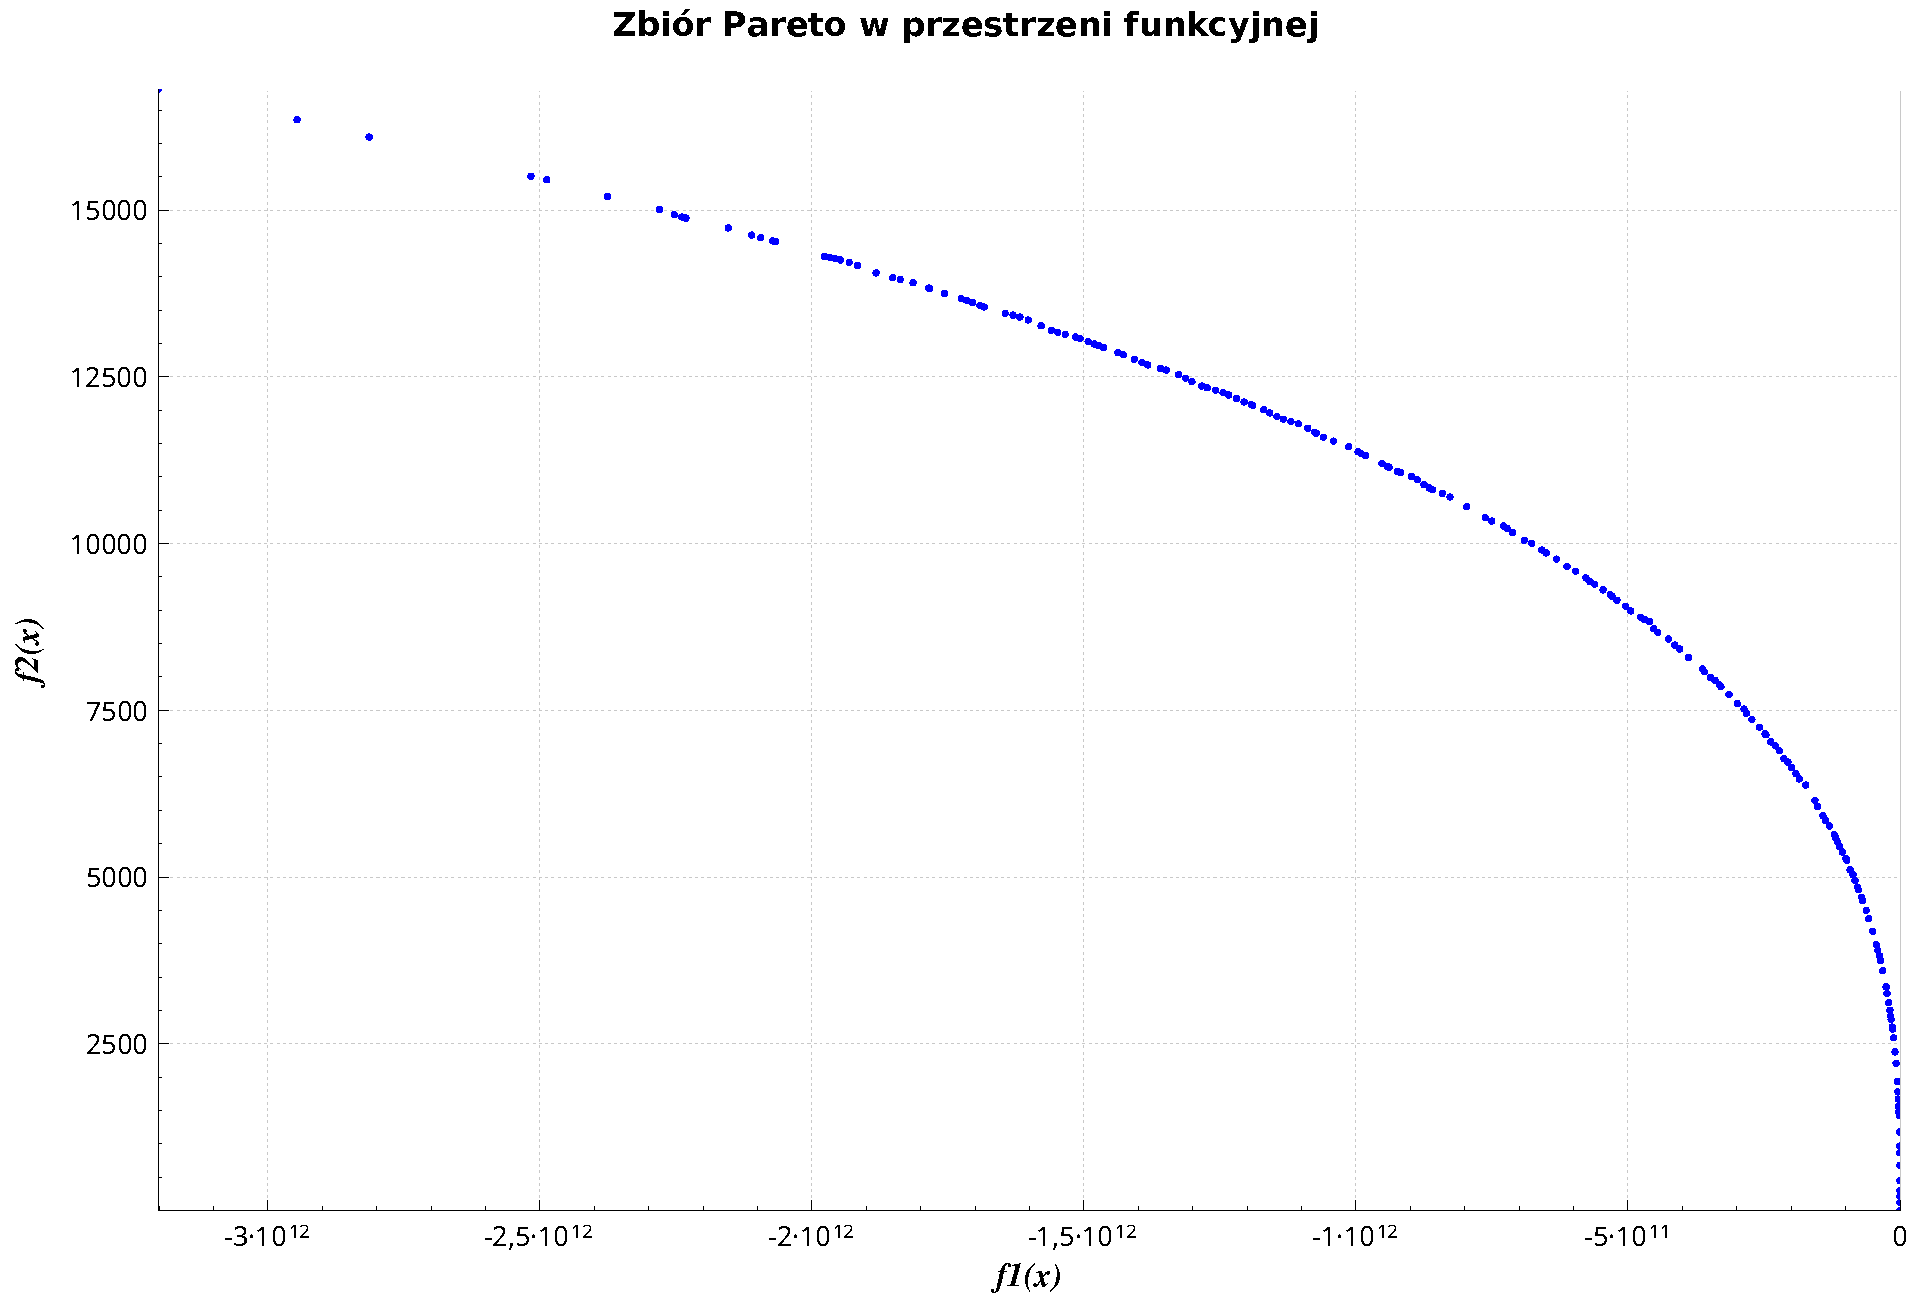
\includegraphics[width=14cm]{rastrigin_goldstein_200_100}
\caption{TBD}
\label{fig:rastrigin_goldstein_200_100}
\end{figure}

\begin{thebibliography}{9}
\bibitem{deb} K. Deb and A. Pratap and S. Agarwal and T. Meyarivan:
\emph{A Fast and Elitist Multiobjective Genetic Algorithm: NSGA–II},
IEEE Transactions on Evolutionary Computation, 2002
\end{thebibliography}

\end{document}